\chapter{Apéndices}

\section{Demostración de $[\hat{a}, \hat{a}^\dagger] = 1$} \label{sec:born1925}


Partimos de las definiciones:

\begin{align}
	\hat{a} &= \sqrt{\frac{m\omega}{2\hbar}}\left(\hat{x} + \frac{i}{m\omega}\hat{p}\right) \\
	\hat{a}^\dagger &= \sqrt{\frac{m\omega}{2\hbar}}\left(\hat{x} - \frac{i}{m\omega}\hat{p}\right)
\end{align}

Calculamos el conmutador $[\hat{a}, \hat{a}^\dagger] = \hat{a}\hat{a}^\dagger - \hat{a}^\dagger\hat{a}$:

\begin{align}
	\hat{a}\hat{a}^\dagger &= \frac{m\omega}{2\hbar}\left(\hat{x} + \frac{i}{m\omega}\hat{p}\right)\left(\hat{x} - \frac{i}{m\omega}\hat{p}\right) \\
	&= \frac{m\omega}{2\hbar}\left(\hat{x}^2 - \frac{i}{m\omega}\hat{x}\hat{p} + \frac{i}{m\omega}\hat{p}\hat{x} + \frac{1}{m^2\omega^2}\hat{p}^2\right) \\
	&= \frac{m\omega}{2\hbar}\hat{x}^2 + \frac{1}{2m\omega\hbar}\hat{p}^2 + \frac{i}{2\hbar}(\hat{p}\hat{x} - \hat{x}\hat{p})
\end{align}

El último término es $-\frac{i}{2\hbar}[\hat{x}, \hat{p}]$. Similarmente:

\begin{align}
	\hat{a}^\dagger\hat{a} &= \frac{m\omega}{2\hbar}\left(\hat{x} - \frac{i}{m\omega}\hat{p}\right)\left(\hat{x} + \frac{i}{m\omega}\hat{p}\right) \\
	&= \frac{m\omega}{2\hbar}\hat{x}^2 + \frac{1}{2m\omega\hbar}\hat{p}^2 + \frac{i}{2\hbar}[\hat{x}, \hat{p}]
\end{align}

Restando:

\begin{equation}
	[\hat{a}, \hat{a}^\dagger] = \hat{a}\hat{a}^\dagger - \hat{a}^\dagger\hat{a} = -\frac{i}{2\hbar}[\hat{x}, \hat{p}] - \frac{i}{2\hbar}[\hat{x}, \hat{p}] = -\frac{i}{\hbar}[\hat{x}, \hat{p}]
\end{equation}

Usando la relación de conmutación canónica de \cite{born1925}:

\begin{equation}
	[\hat{x}, \hat{p}] = i\hbar
\end{equation}

Obtenemos:

\begin{equation}
	[\hat{a}, \hat{a}^\dagger] = -\frac{i}{\hbar}(i\hbar) = -i^2 = 1
\end{equation}

\begin{equation}
	\boxed{[\hat{a}, \hat{a}^\dagger] = 1}
\end{equation}	
	
% APÉNDICE NUEVO: Factorización algebraica del hamiltoniano

 \section{Factorización algebraica del hamiltoniano}
 \label{sec:factorizacion}

 Sustituyendo las expresiones de $\hat{x}$ y $\hat{p}$ en términos de los
 operadores escalera:

\begin{equation}
 \hat{p}^2 = -\frac{m\omega\hbar}{2}(\hat{a}^\dagger - \hat{a})^2
           = -\frac{m\omega\hbar}{2}(\hat{a}^{\dagger 2} - \hat{a}^\dagger\hat{a}
             - \hat{a}\hat{a}^\dagger + \hat{a}^2)
\end{equation}

\begin{equation}
 \hat{x}^2 = \frac{\hbar}{2m\omega}(\hat{a} + \hat{a}^\dagger)^2
           = \frac{\hbar}{2m\omega}(\hat{a}^2 + \hat{a}\hat{a}^\dagger + \hat{a}^\dagger\hat{a} + \hat{a}^{\dagger 2})
\end{equation}

Sumando los términos $\frac{\hat{p}^2}{2m} + \frac{1}{2}m\omega^2\hat{x}^2$ y usando $[\hat{a},\hat{a}^\dagger]=1$, es decir,
$\hat{a}\hat{a}^\dagger = \hat{a}^\dagger\hat{a} + 1$:

\begin{equation}
\hat{H} = \hbar\omega\left(\hat{a}^\dagger\hat{a} + \frac{1}{2}\right)
         = \hbar\omega\left(\hat{N} + \frac{1}{2}\right)
\end{equation}

 Los términos cruzados $\hat{a}^2$ y $\hat{a}^{\dagger 2}$ se cancelan,
 y los términos $\hat{a}\hat{a}^\dagger + \hat{a}^\dagger\hat{a}
 = 2\hat{N} + 1$ producen el resultado final.


\section{Constantes de normalización: $\hat{a}^\dagger|n\rangle = \sqrt{n+1}|n+1\rangle$} \label{sec:normalizacion1}

Queremos determinar la constante de proporcionalidad cuando $\hat{a}^\dagger$ actúa sobre $|n\rangle$.

Sabemos que $\hat{a}^\dagger|n\rangle$ es proporcional a $|n+1\rangle$:

\begin{equation}
	\hat{a}^\dagger|n\rangle = c|n+1\rangle
\end{equation}

Para encontrar $c$, calculamos la norma al cuadrado:

\begin{equation}
	||\hat{a}^\dagger|n\rangle||^2 = \langle n|\hat{a}\hat{a}^\dagger|n\rangle
\end{equation}

Usando la relación de conmutación $\hat{a}\hat{a}^\dagger = \hat{a}^\dagger\hat{a} + 1$:

\begin{align}
	||\hat{a}^\dagger|n\rangle||^2 &= \langle n|(\hat{a}^\dagger\hat{a} + 1)|n\rangle \tag{A.14}\\
	&= \langle n|\hat{N}|n\rangle + \langle n|n\rangle \quad \text{(donde } \hat{N} = \hat{a}^\dagger\hat{a}\text{)} \tag{A.15}\\
	&= n + 1 \tag{A.16}
\end{align}

Por otro lado, si $\hat{a}^\dagger|n\rangle = c|n+1\rangle$:

\begin{equation}
	||\hat{a}^\dagger|n\rangle||^2 = |c|^2
\end{equation}

Igualando: $|c|^2 = n + 1$, entonces $c = \sqrt{n+1}$ (tomamos la raíz positiva por convención).

\textbf{Resultado:}

\begin{equation}
	\boxed{\hat{a}^\dagger|n\rangle = \sqrt{n+1}|n+1\rangle}
\end{equation}

	

\section{Constantes de normalización: $\hat{a}|n\rangle = \sqrt{n}|n-1\rangle$} \label{sec:normalizacion2}

De manera análoga, para $\hat{a}|n\rangle = d|n-1\rangle$:

\begin{align}
	||\hat{a}|n\rangle||^2 &= \langle n|\hat{a}^\dagger\hat{a}|n\rangle \\
	&= \langle n|\hat{N}|n\rangle \\
	&= n
\end{align}

Por lo tanto: $|d|^2 = n \implies d = \sqrt{n}$

\textbf{Resultado:}

\begin{equation}
	\boxed{\hat{a}|n\rangle = \sqrt{n}|n-1\rangle}
\end{equation}

\begin{table}[h]
	\centering
	\caption{Acción de los operadores escalera sobre autoestados}
	\label{tab:operadores_escalera}
	\begin{tabular}{ccc}
		\hline
		\textbf{Estado inicial} & \textbf{Operador creación} & \textbf{Operador aniquilación} \\
		& $\hat{a}^\dagger|n\rangle$ & $\hat{a}|n\rangle$ \\
		\hline
		$|0\rangle$ & $\sqrt{1}|1\rangle = |1\rangle$ & $0$ \\
		$|1\rangle$ & $\sqrt{2}|2\rangle$ & $\sqrt{1}|0\rangle = |0\rangle$ \\
		$|2\rangle$ & $\sqrt{3}|3\rangle$ & $\sqrt{2}|1\rangle$ \\
		$|3\rangle$ & $\sqrt{4}|4\rangle = 2|4\rangle$ & $\sqrt{3}|2\rangle$ \\
		$|n\rangle$ & $\sqrt{n+1}|n+1\rangle$ & $\sqrt{n}|n-1\rangle$ \\
		\hline
	\end{tabular}
\end{table}



\section{Polinomios de Hermite} \label{sec:hermite}

Los polinomios de Hermite $H_n(\xi)$ aparecen en las autofunciones del oscilador armónico cuántico. Este apéndice presenta sus propiedades esenciales.

\subsection{Definición}

Los polinomios de Hermite se definen mediante la fórmula de Rodrigues:

\begin{equation}
	H_n(\xi) = (-1)^n e^{\xi^2} \frac{d^n}{d\xi^n} e^{-\xi^2}
\end{equation}



\begin{figure}[h!]
	\centering
	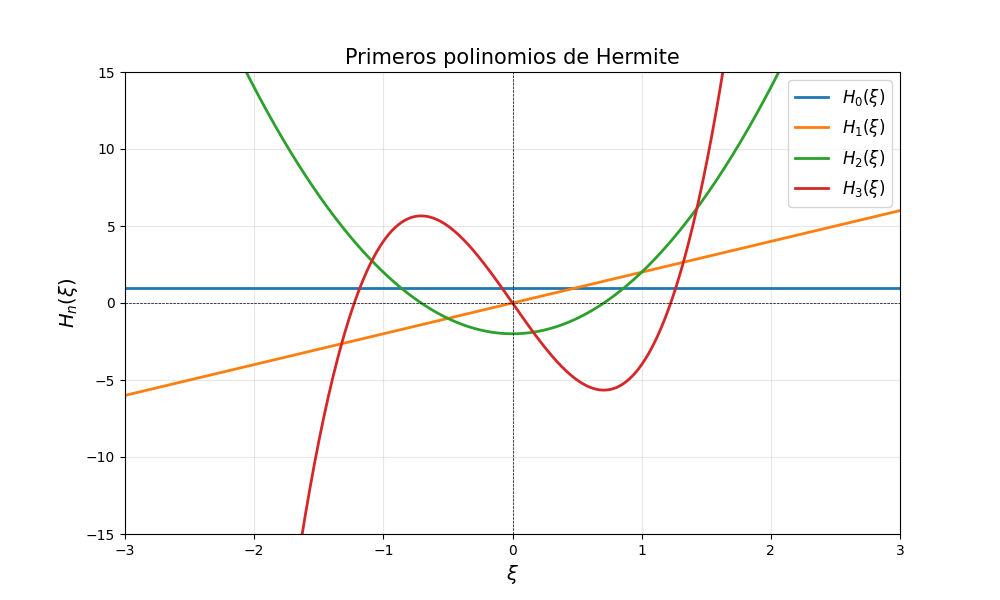
\includegraphics[width=0.9\linewidth]{hermite}
	\caption{Ejemplos de polinomios de Hermite $H_0, H_1, H_2, H_3$}
	\label{fig:hermite}
\end{figure}



\subsection{Primeros polinomios}

\begin{align}
	H_0(\xi) &= 1 \\
	H_1(\xi) &= 2\xi \\
	H_2(\xi) &= 4\xi^2 - 2 \\
	H_3(\xi) &= 8\xi^3 - 12\xi \\
	H_4(\xi) &= 16\xi^4 - 48\xi^2 + 12
\end{align}

\textbf{Propiedades generales:}
\begin{itemize}
	\item $H_n(\xi)$ es un polinomio de grado $n$
	\item El coeficiente del término de mayor grado es $2^n$
	\item Paridad: $H_n(-\xi) = (-1)^n H_n(\xi)$
\end{itemize}

\subsection{Relación de recurrencia}

Los polinomios se pueden generar mediante:

\begin{equation}
	H_{n+1}(\xi) = 2\xi H_n(\xi) - 2n H_{n-1}(\xi)
\end{equation}

Esta relación permite calcular $H_{n+1}$ conociendo $H_n$ y $H_{n-1}$.

\subsection{Ortogonalidad}

Los polinomios de Hermite son ortogonales con peso gaussiano:

\begin{equation}
	\int_{-\infty}^{\infty} H_n(\xi) H_m(\xi) e^{-\xi^2} d\xi = \begin{cases}
		0 & \text{si } n \neq m \\
		\sqrt{\pi} \, 2^n n! & \text{si } n = m
	\end{cases}
\end{equation}

Esta propiedad garantiza la ortonormalidad de las autofunciones del OAC cuando se incluye la constante de normalización apropiada:

\begin{equation}
	A_n = \left(\frac{m\omega}{\pi\hbar}\right)^{1/4} \frac{1}{\sqrt{2^n n!}}
\end{equation}

\subsection{Consecuencias para las autofunciones}

\textbf{Paridad:} Como $H_n(-\xi) = (-1)^n H_n(\xi)$, las autofunciones tienen paridad bien definida:
\begin{equation}
	\psi_n(-x) = (-1)^n \psi_n(x)
\end{equation}

Estados pares ($n$ par): funciones simétricas

Estados impares ($n$ impar): funciones antisimétricas

\textbf{Número de nodos:} El polinomio $H_n(\xi)$ tiene exactamente $n$ ceros reales. Por lo tanto, $\psi_n(x)$ tiene exactamente $n$ nodos.

